\documentclass{article}

\usepackage{amsmath}
\usepackage{amssymb}
\usepackage{graphicx}

\begin{document}


Ivan Lin\newline{}
Dr. Esther Arkin\newline{}
AMS301\newline{}
3/3/17

\begin{center}
  Homework 5b
\end{center}

\underline{Problem B}
(a). Determine the DFS tree of K6.
(b). Determine the BFS tree of K6.

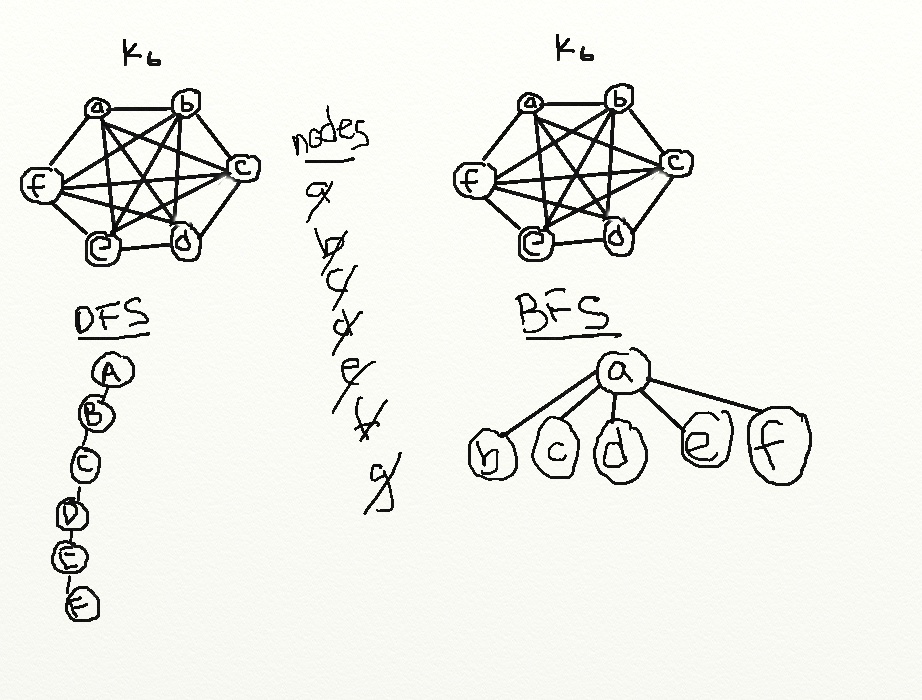
\includegraphics[width=\textwidth]{problemb.png}

\underline{Problem C} 

True or False? If true, give a short proof. If false, give a counterexample:
(a). For any connected graph G, all internal nodes of the BFS tree on G have the same number of children.\newline{}
False\newline{}
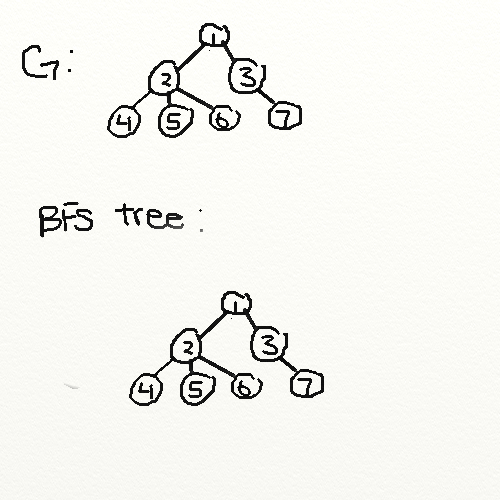
\includegraphics[width=\textwidth]{problemca.png}
(b). For any connected graph G, the DFS tree on G and the BFS tree on G have the same number of edges.\newline{}
True - any search tree of a graph will have the same number of vertices $n$ as the graph. Since a tree is minimally connected and have $n-1$ edges, all trees composed of the same number of nodes will always have the same number of edges.\newline{}
(c). The height of a DFS tree starting at node A must be greater than or equal to the height of a BFS tree
starting at the same node A.\newline{}
True - a breadth-first-search tree will always be the smallest possible height. The bredth first search follows a first-in-first-out structure, meaning that older nodes will be filled before newer nodes are filled, so higher levels are always completed first before nodes are added to lower levels. Since it uses the minimum possible height for a tree, any other tree with the same set of nodes will have a height greater than or equal to that of the BFS tree.\newline{}
(d). The height of a DFS tree starting at node B must be greater than or equal to the height of a BFS tree
starting at some other node A\newline{}
False - \newline{}
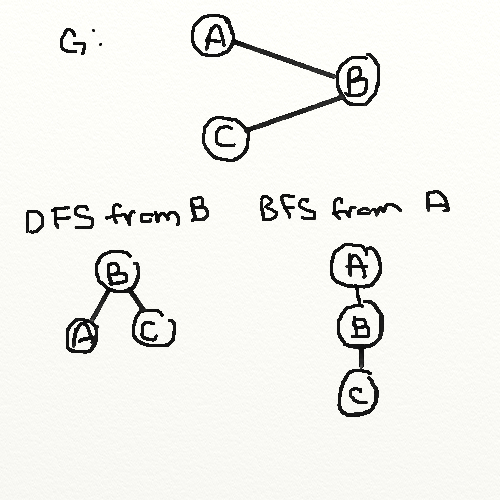
\includegraphics[width=\textwidth]{problemcd.png}
\end{document}
